\documentclass[a4paper,14pt]{extarticle}

\usepackage[utf8x]{inputenc}
\usepackage[T1]{fontenc}
\usepackage[russian]{babel}
\usepackage{hyperref}
\usepackage{indentfirst}
\usepackage{here}
\usepackage{array}
\usepackage{graphicx}
\usepackage{grffile}
\usepackage{caption}
\usepackage{subcaption}
\usepackage{chngcntr}
\usepackage{amsmath}
\usepackage{amssymb}
\usepackage{pgfplots}
\usepackage{pgfplotstable}
\usepackage[left=2cm,right=2cm,top=2cm,bottom=2cm,bindingoffset=0cm]{geometry}
\usepackage{multicol}
\usepackage{multirow}
\usepackage{titlesec}
\usepackage{listings}
\usepackage{color}
\usepackage{longtable}
\usepackage{enumitem}
\usepackage{cmap}
\usepackage{tikz}

\usetikzlibrary{shapes,arrows}

\definecolor{green}{rgb}{0,0.6,0}
\definecolor{gray}{rgb}{0.5,0.5,0.5}
\definecolor{purple}{rgb}{0.58,0,0.82}

\lstset{
	language={SQL},
	inputpath={../},
	backgroundcolor=\color{white},
	commentstyle=\color{green},
	keywordstyle=\color{blue},
	numberstyle=\scriptsize\color{gray},
	stringstyle=\color{purple},
	basicstyle=\small,
	breakatwhitespace=false,
	breaklines=true,
	captionpos=b,
	keepspaces=true,
	numbers=left,
	numbersep=5pt,
	showspaces=false,
	showstringspaces=false,
	showtabs=false,
	tabsize=8,
	frame=single,
}

\renewcommand{\le}{\ensuremath{\leqslant}}
\renewcommand{\leq}{\ensuremath{\leqslant}}
\renewcommand{\ge}{\ensuremath{\geqslant}}
\renewcommand{\geq}{\ensuremath{\geqslant}}
\renewcommand{\epsilon}{\ensuremath{\varepsilon}}
\renewcommand{\phi}{\ensuremath{\varphi}}
\renewcommand{\thefigure}{\arabic{figure}}
\def\code#1{\texttt{#1}}

\titleformat*{\section}{\large\bfseries} 
\titleformat*{\subsection}{\normalsize\bfseries} 
\titleformat*{\subsubsection}{\normalsize\bfseries} 
\titleformat*{\paragraph}{\normalsize\bfseries} 
\titleformat*{\subparagraph}{\normalsize\bfseries} 

\counterwithin{figure}{section}
\counterwithin{equation}{section}
\counterwithin{table}{section}
\newcommand{\sign}[1][5cm]{\makebox[#1]{\hrulefill}}
\newcommand{\equipollence}{\quad\Leftrightarrow\quad}
\newcommand{\no}[1]{\overline{#1}}
\graphicspath{{../}}
\captionsetup{justification=centering,margin=1cm}
\def\arraystretch{1.3}
\setlength\parindent{5ex}
\titlelabel{\thetitle.\quad}

\setitemize{itemsep=0em}
\setenumerate{itemsep=0em}

\tikzstyle{startstop} = [
	rectangle,
	align=center,
	rounded corners,
	text width=10em,
	text centered,
	draw=black
]
\tikzstyle{process} = [
	rectangle,
	align=center,
	text width=20em,
	text centered,
	draw=black
]
\tikzstyle{decision} = [
	diamond,
	aspect=4,
	align=center,
	inner sep=0pt,
	text width=10em,
	text centered,
	node distance=5em,
	draw=black
]
\tikzstyle{line} = [
	draw=black,
	thick,
	->,
	>=stealth,
	-latex'
]

\begin{document}

\begin{titlepage}
\begin{center}
	САНКТ-ПЕТЕРБУРГСКИЙ ПОЛИТЕХНИЧЕСКИЙ УНИВЕРСИТЕТ\\ ПЕТРА ВЕЛИКОГО\\[0.3cm]
	\par\noindent\rule{10cm}{0.4pt}\\[0.3cm]
	Институт компьютерных наук и технологий \\[0.3cm]
	Кафедра компьютерных систем и программных технологий\\[4cm]
	
	Отчет по лабораторной работе № 1\\[3mm]
	Дисциплина: <<Базы данных>>\\[3mm]
	Тема: <<Разработка структуры БД>>\\[7cm]
\end{center}

\begin{flushleft}
	\hspace*{5mm} Выполнил студент гр. 43501/3  \hspace*{2.5cm}\sign[3cm]\hspace*{3.0mm} А.Ю. Ламтев\\
	\hspace*{10.4cm} (подпись)\\[3mm]
	\hspace*{5mm} Преподаватель \hspace*{6.0cm}\sign[3cm]\hspace*{2mm} А.В. Мяснов\\
	\hspace*{10.4cm} (подпись)\\[3mm]
	\hspace*{11.1cm} <<\sign[7mm]>> \sign[27mm] \the\year\hspace{1mm} г.
\end{flushleft}

\vfill

\begin{center}
	Санкт-Петербург\\
	\the\year
\end{center}
\end{titlepage}
\addtocounter{page}{1}

\tableofcontents
\newpage

\section{Цели работы}

Познакомиться с основами проектирования схемы БД, способами организации данных в SQL-БД. 

\section{Программа работы}

\begin{enumerate}
	\item Создание проекта для работы в GitLab.
	\item Выбор задания (предметной области), описание набора данных и требований к хранимым данным в свободном формате в wiki своего проекта в GitLab.
	\item Формирование в свободном формате (предпочтительно в виде графической схемы) cхемы БД, соответствующей заданию. Должно получиться не менее 7 таблиц.
	\item Согласование с преподавателем схемы БД. Обоснование принятых решений и соответствия требованиям выбранного задания. 
	\item Выкладывание схемы БД в свой проект в GitLab.
	\item Демонстрация результатов преподавателю.
\end{enumerate}


\section{Задание}

В качестве предметной области был выбран \textit{сетевой сервис фильмов}.

Зарегистрированный пользователь сервиса может купить конкретные фильмы или сериалы на постоянной основе или оформить подписку на весь видеоконтент, предоставляемый сервисом, на определённый срок. Контент локазизован на все основные языки. Подписка может быть автоматически продляемой по истечении срока действия. При выборе фильма или сериала пользователь может ознакомиться с описанием, которое содержит режиссёра, рейтинг \code{IMDB}, дату выпуска, и в случае сериала количество сезонов. Для регистрации в сервисе пользователю нужно указать логин, пароль, адрес электронной почты, дату рождения, пол, имя и фамилию. Также пользователь может запросить выписку по всем своим покупкам и подпискам.

\section{Схема БД}
 
На рис. \ref{fig:movie-service-diagram} изображена \code{ER} диаграмма БД, соответствующей заданию.

\begin{figure}[H]
	\centering
	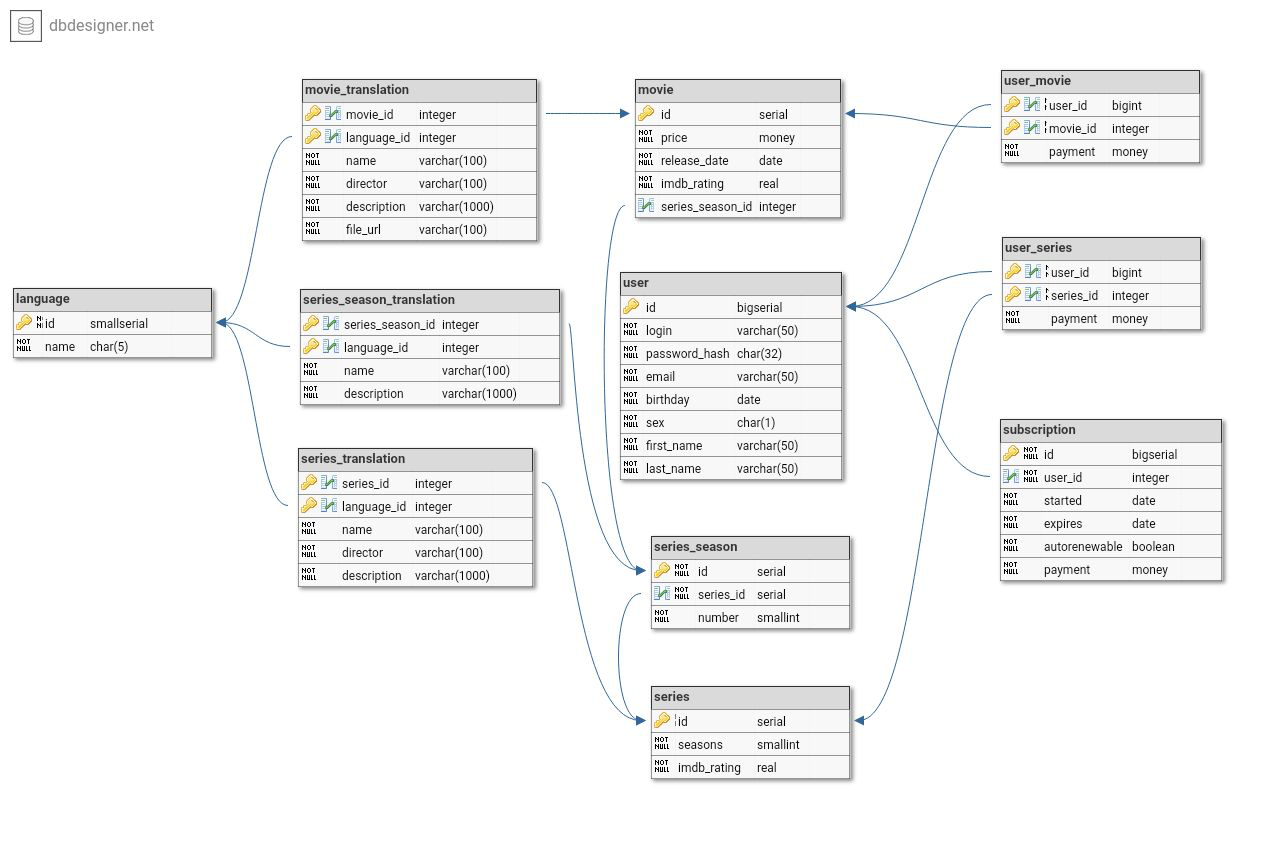
\includegraphics[width=1.0\textwidth]{diagrams/movie-service-diagram}
	\caption{\code{ER} диаграмма БД}
	\label{fig:movie-service-diagram}
\end{figure}

\section{Выводы}

В результате работы была сформулирована предметная область --- \textit{сетевой сервис фильмов} --- которая будет использоваться и в следующих лабораторных работах данного курса. В соответствии с предметной областью
была разработана и продемонстрирована в виде \code{ER} диаграммы модель данных.

Таким образом, было проведено ознакомление с основами проектирования схемы БД и способами организации данных в SQL-БД.

\end{document}
